\chapter{Testes empíricos e análise dos resultados}

Neste capítulo serão apresentados os testes propostos para validação do método
de classificação descrito nesta monografia, bem como a compilação dos
resultados obtidos acompanhados de breves observações.

\section{Roteiro e fundamentação do teste proposto}

Este trabalho propõe como teste de validação para técnica de classificação
descrita nos capítulos anteriores um esquema simples de comparação de
expectativas, haverá um grupo de imagens previamente classificado por agentes
humanos, e outra classificação, para este mesmo grupo de imagens, gerada pela
técnica aqui proposta, deste modo, será possível efetuar a comparação entre a
expectativa, isto é, as classes que idealmente devem ser geradas, representadas
pela classificação humana das imagens, com as classes fornecidas pela técnica
baseada nas redes de Kohonen.

O objetivo do teste é avaliar a quantidade e a pertinência das classes, ou seja,
se o mesmo número de classes aparece em ambos as classificações e se as classes
geradas pelo método proposto possuem correspondência com as classes definidas
pelos agentes humanos, mais especificamente, se as imagens estão agrupadas pelo
método baseado nas redes de Kohonen do mesmo modo, ou de modo muito semelhante,
como foram agrupadas pelos agentes humanos.

\section{Especificação do conjunto de imagens e das classes de controle}
\label{sec:conjunto_de_imagens}

O conjunto de imagens utilizada para a execução do teste é o
\textit{Columbia Object Image Library} (COIL-100), um conjunto de 100
objetos em 7200 poses
diferentes \cite{Coil}. Destes 100, foram escolhidas 91 imagens de diferentes objetos para
compor o teste. Foram identificadas 15 classes para estas imagens, cada classe possui
imagens em poses com variações de translação, rotação e escala para o mesmo tipo
de objeto, afim de confrontar as premissas da Seção \ref{sec:momentos_desc} no
contexto do processo de classificação.

As classes identificadas foram nomeadas e apresentam as seguintes imagens:

\begin{table}[H]
  \centering
  \caption{Grupo A (animais de brinquedo).}
  \tabulinesep =_0.5em^0.5em
  \everyrow{\tabucline[0.4pt]-}
  \begin{tabu}{|cccccc|}
    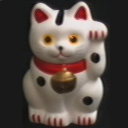
\includegraphics[width=0.1\textwidth,height=0.1\textwidth]{imagens/coil_100/animais_brinquedos/obj14__0.png} &
    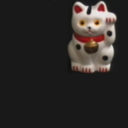
\includegraphics[width=0.1\textwidth,height=0.1\textwidth]{imagens/coil_100/animais_brinquedos/obj14__0_1.png} &
    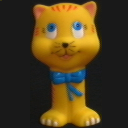
\includegraphics[width=0.1\textwidth,height=0.1\textwidth]{imagens/coil_100/animais_brinquedos/obj17__0.png} &
    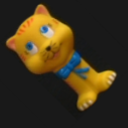
\includegraphics[width=0.1\textwidth,height=0.1\textwidth]{imagens/coil_100/animais_brinquedos/obj17__0_1.png} &
    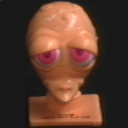
\includegraphics[width=0.1\textwidth,height=0.1\textwidth]{imagens/coil_100/animais_brinquedos/obj20__0.png} &
    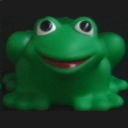
\includegraphics[width=0.1\textwidth,height=0.1\textwidth]{imagens/coil_100/animais_brinquedos/obj28__275.png}
    \\
    \scriptsize{obj01.jpg} & \scriptsize{obj02.jpg} & \scriptsize{obj03.jpg} &
    \scriptsize{obj04.jpg} & \scriptsize{obj05.jpg} & \scriptsize{obj06.jpg}
    \\
    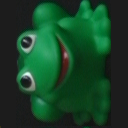
\includegraphics[width=0.1\textwidth,height=0.1\textwidth]{imagens/coil_100/animais_brinquedos/obj28__275_1.png} &
    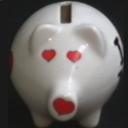
\includegraphics[width=0.1\linewidth,height=0.1\linewidth]{imagens/coil_100/animais_brinquedos/obj48__265.png} &
    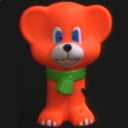
\includegraphics[width=0.1\linewidth,height=0.1\linewidth]{imagens/coil_100/animais_brinquedos/obj52__0.png} &
    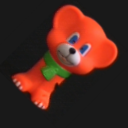
\includegraphics[width=0.1\linewidth,height=0.1\linewidth]{imagens/coil_100/animais_brinquedos/obj52__0_1.png} &
    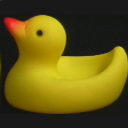
\includegraphics[width=0.1\linewidth,height=0.1\linewidth]{imagens/coil_100/animais_brinquedos/obj74__0.png} &
    \\
    \scriptsize{obj07.jpg} & \scriptsize{obj08.jpg} & \scriptsize{obj09.jpg} &
    \scriptsize{obj10.jpg} & \scriptsize{obj11.jpg} &
  \end{tabu}
\end{table}

\begin{table}[H]
  \centering
  \caption{Grupo B (barquinhos de brinquedo).}
  \tabulinesep =_0.5em^0.5em
  \everyrow{\tabucline[0.4pt]-}
  \begin{tabu}{|ccc|}
    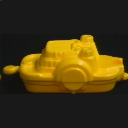
\includegraphics[width=0.1\textwidth,height=0.1\textwidth]{imagens/coil_100/barquinhos_brinquedos/obj3__0.png} &
    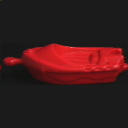
\includegraphics[width=0.1\textwidth,height=0.1\textwidth]{imagens/coil_100/barquinhos_brinquedos/obj38__0.png} &
    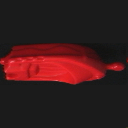
\includegraphics[width=0.1\textwidth,height=0.1\textwidth]{imagens/coil_100/barquinhos_brinquedos/obj38__0_1.png}
    \\
    \scriptsize{obj12.jpg} & \scriptsize{obj13.jpg} & \scriptsize{obj14.jpg}
    \\
    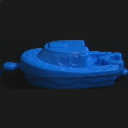
\includegraphics[width=0.1\textwidth,height=0.1\textwidth]{imagens/coil_100/barquinhos_brinquedos/obj42__0.png} &
    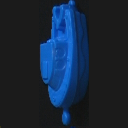
\includegraphics[width=0.1\textwidth,height=0.1\textwidth]{imagens/coil_100/barquinhos_brinquedos/obj42__0_1.png} &
    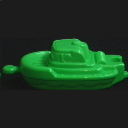
\includegraphics[width=0.1\textwidth,height=0.1\textwidth]{imagens/coil_100/barquinhos_brinquedos/obj78__0.png}
    \\
    \scriptsize{obj15.jpg} & \scriptsize{obj16.jpg} & \scriptsize{obj17.jpg}
  \end{tabu}
\end{table}

\begin{table}[H]
  \centering
  \caption{Grupo C (boias).}
  \tabulinesep =_0.5em^0.5em
  \everyrow{\tabucline[0.4pt]-}
  \begin{tabu}{|ccc|}
    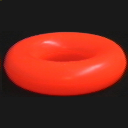
\includegraphics[width=0.1\textwidth,height=0.1\textwidth]{imagens/coil_100/boias/obj47__0.png} &
    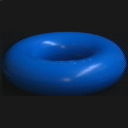
\includegraphics[width=0.1\textwidth,height=0.1\textwidth]{imagens/coil_100/boias/obj94__0.png} &
    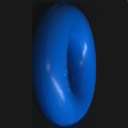
\includegraphics[width=0.1\textwidth,height=0.1\textwidth]{imagens/coil_100/boias/obj94__0_1.png}
    \\
    \scriptsize{obj18.jpg} & \scriptsize{obj19.jpg} & \scriptsize{obj20.jpg}
  \end{tabu}
\end{table}

\begin{table}[H]
  \centering
  \caption{Grupo D (caixas).}
  \tabulinesep =_0.5em^0.5em
  \everyrow{\tabucline[0.4pt]-}
  \begin{tabu}{|ccccccc|}
    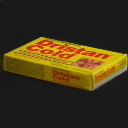
\includegraphics[width=0.1\textwidth,height=0.1\textwidth]{imagens/coil_100/caixas/obj1__35.png} &
    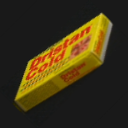
\includegraphics[width=0.1\textwidth,height=0.1\textwidth]{imagens/coil_100/caixas/obj1__35_1.png} &
    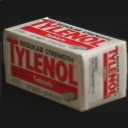
\includegraphics[width=0.1\textwidth,height=0.1\textwidth]{imagens/coil_100/caixas/obj31__45.png} &
    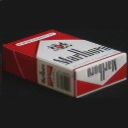
\includegraphics[width=0.1\textwidth,height=0.1\textwidth]{imagens/coil_100/caixas/obj46__45.png} &
    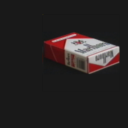
\includegraphics[width=0.1\textwidth,height=0.1\textwidth]{imagens/coil_100/caixas/obj46__45_1.png} &
    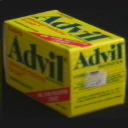
\includegraphics[width=0.1\textwidth,height=0.1\textwidth]{imagens/coil_100/caixas/obj54__55.png} &
    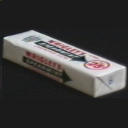
\includegraphics[width=0.1\textwidth,height=0.1\textwidth]{imagens/coil_100/caixas/obj67__50.png}
    \\
    \scriptsize{obj21.jpg} & \scriptsize{obj22.jpg} & \scriptsize{obj23.jpg} &
    \scriptsize{obj24.jpg} & \scriptsize{obj25.jpg} & \scriptsize{obj26.jpg} &
    \scriptsize{obj27.jpg}
    \\
    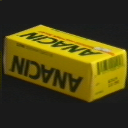
\includegraphics[width=0.1\textwidth,height=0.1\textwidth]{imagens/coil_100/caixas/obj79__45.png} &
    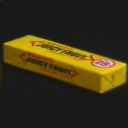
\includegraphics[width=0.1\textwidth,height=0.1\textwidth]{imagens/coil_100/caixas/obj84__45.png} &
    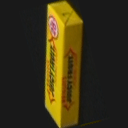
\includegraphics[width=0.1\textwidth,height=0.1\textwidth]{imagens/coil_100/caixas/obj84__45_1.png} &
    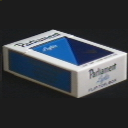
\includegraphics[width=0.1\textwidth,height=0.1\textwidth]{imagens/coil_100/caixas/obj96__45.png} &
    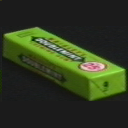
\includegraphics[width=0.1\textwidth,height=0.1\textwidth]{imagens/coil_100/caixas/obj98__55.png} &
    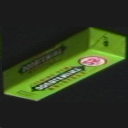
\includegraphics[width=0.1\textwidth,height=0.1\textwidth]{imagens/coil_100/caixas/obj98__55_1.png} &
    \\
    \scriptsize{obj28.jpg} & \scriptsize{obj29.jpg} & \scriptsize{obj30.jpg} &
    \scriptsize{obj31.jpg} & \scriptsize{obj32.jpg} & \scriptsize{obj33.jpg} &
  \end{tabu}
\end{table}

\begin{table}[H]
  \centering
  \caption{Grupo E (carrinhos de brinquedo).}
  \tabulinesep =_0.5em^0.5em
  \everyrow{\tabucline[0.4pt]-}
  \begin{tabu}{|ccccccc|}
    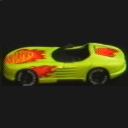
\includegraphics[width=0.1\textwidth,height=0.1\textwidth]{imagens/coil_100/carrinhos_brinquedos/obj6__0.png} &
    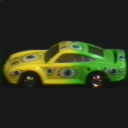
\includegraphics[width=0.1\textwidth,height=0.1\textwidth]{imagens/coil_100/carrinhos_brinquedos/obj8__0.png} &
    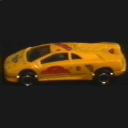
\includegraphics[width=0.1\textwidth,height=0.1\textwidth]{imagens/coil_100/carrinhos_brinquedos/obj15__0.png} &
    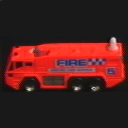
\includegraphics[width=0.1\textwidth,height=0.1\textwidth]{imagens/coil_100/carrinhos_brinquedos/obj19__0.png} &
    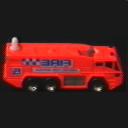
\includegraphics[width=0.1\textwidth,height=0.1\textwidth]{imagens/coil_100/carrinhos_brinquedos/obj19__0_1.png} &
    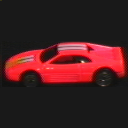
\includegraphics[width=0.1\textwidth,height=0.1\textwidth]{imagens/coil_100/carrinhos_brinquedos/obj23__0.png} &
    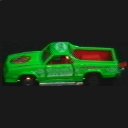
\includegraphics[width=0.1\textwidth,height=0.1\textwidth]{imagens/coil_100/carrinhos_brinquedos/obj27__0.png}
    \\
    \scriptsize{obj34.jpg} & \scriptsize{obj35.jpg} & \scriptsize{obj36.jpg} &
    \scriptsize{obj37.jpg} & \scriptsize{obj38.jpg} & \scriptsize{obj39.jpg} &
    \scriptsize{obj40.jpg}
    \\
    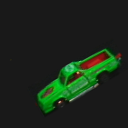
\includegraphics[width=0.1\textwidth,height=0.1\textwidth]{imagens/coil_100/carrinhos_brinquedos/obj27__0_1.png} &
    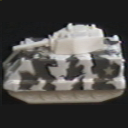
\includegraphics[width=0.1\textwidth,height=0.1\textwidth]{imagens/coil_100/carrinhos_brinquedos/obj37__0.png} &
    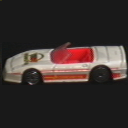
\includegraphics[width=0.1\textwidth,height=0.1\textwidth]{imagens/coil_100/carrinhos_brinquedos/obj69__0.png} &
    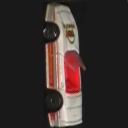
\includegraphics[width=0.1\textwidth,height=0.1\textwidth]{imagens/coil_100/carrinhos_brinquedos/obj69__0_1.png} &
    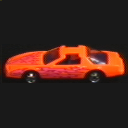
\includegraphics[width=0.1\textwidth,height=0.1\textwidth]{imagens/coil_100/carrinhos_brinquedos/obj76__0.png} &
    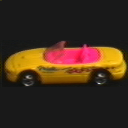
\includegraphics[width=0.1\textwidth,height=0.1\textwidth]{imagens/coil_100/carrinhos_brinquedos/obj91__0.png} &
    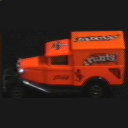
\includegraphics[width=0.1\textwidth,height=0.1\textwidth]{imagens/coil_100/carrinhos_brinquedos/obj100__0.png}
    \\
    \scriptsize{obj41.jpg} & \scriptsize{obj42.jpg} & \scriptsize{obj43.jpg} &
    \scriptsize{obj44.jpg} & \scriptsize{obj45.jpg} & \scriptsize{obj46.jpg} &
    \scriptsize{obj47.jpg}
  \end{tabu}
\end{table}

\begin{table}[H]
  \centering
  \caption{Grupo F (chícaras).}
  \tabulinesep =_0.5em^0.5em
  \everyrow{\tabucline[0.4pt]-}
  \begin{tabu}{|cccccc|}
    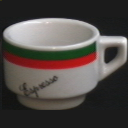
\includegraphics[width=0.1\textwidth,height=0.1\textwidth]{imagens/coil_100/chicaras/obj10__0.png} &
    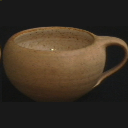
\includegraphics[width=0.1\textwidth,height=0.1\textwidth]{imagens/coil_100/chicaras/obj11__0.png} &
    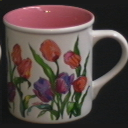
\includegraphics[width=0.1\textwidth,height=0.1\textwidth]{imagens/coil_100/chicaras/obj16__0.png} &
    \includegraphics[width=0.1\textwidth,height=0.1\textwidth]{imagens/coil_100/chicaras/obj16__0_1.png} &
    \includegraphics[width=0.1\textwidth,height=0.1\textwidth]{imagens/coil_100/chicaras/obj43__0.png} &
    \includegraphics[width=0.1\textwidth,height=0.1\textwidth]{imagens/coil_100/chicaras/obj43__0_1.png}
    \\
    \scriptsize{obj48.jpg} & \scriptsize{obj49.jpg} & \scriptsize{obj50.jpg} &
    \scriptsize{obj51.jpg} & \scriptsize{obj52.jpg} & \scriptsize{obj53.jpg}
    \\
    \includegraphics[width=0.1\textwidth,height=0.1\textwidth]{imagens/coil_100/chicaras/obj45__0.png} &
    \includegraphics[width=0.1\textwidth,height=0.1\textwidth]{imagens/coil_100/chicaras/obj59__0.png} &
    \includegraphics[width=0.1\textwidth,height=0.1\textwidth]{imagens/coil_100/chicaras/obj59__0_1.png} &
    \includegraphics[width=0.1\textwidth,height=0.1\textwidth]{imagens/coil_100/chicaras/obj81__0.png} &
    \includegraphics[width=0.1\textwidth,height=0.1\textwidth]{imagens/coil_100/chicaras/obj89__0.png} &
    \includegraphics[width=0.1\textwidth,height=0.1\textwidth]{imagens/coil_100/chicaras/obj97__0.png}
    \\
    \scriptsize{obj54.jpg} & \scriptsize{obj55.jpg} & \scriptsize{obj56.jpg} &
    \scriptsize{obj57.jpg} & \scriptsize{obj58.jpg} & \scriptsize{obj59.jpg}
  \end{tabu}
\end{table}

\begin{table}[H]
  \centering
  \caption{Grupo G (embalagens cilíndricas).}
  \tabulinesep =_0.5em^0.5em
  \everyrow{\tabucline[0.4pt]-}
  \begin{tabu}{|cccccc|}
    \includegraphics[width=0.1\textwidth,height=0.1\textwidth]{imagens/coil_100/embalagens_cilindricas/obj7__0.png} &
    \includegraphics[width=0.1\textwidth,height=0.1\textwidth]{imagens/coil_100/embalagens_cilindricas/obj26__0.png} &
    \includegraphics[width=0.1\textwidth,height=0.1\textwidth]{imagens/coil_100/embalagens_cilindricas/obj26__0_1.png} &
    \includegraphics[width=0.1\textwidth,height=0.1\textwidth]{imagens/coil_100/embalagens_cilindricas/obj29__0.png} &
    \includegraphics[width=0.1\textwidth,height=0.1\textwidth]{imagens/coil_100/embalagens_cilindricas/obj32__0.png} &
    \includegraphics[width=0.1\textwidth,height=0.1\textwidth]{imagens/coil_100/embalagens_cilindricas/obj49__0.png}
    \\
    \scriptsize{obj60.jpg} & \scriptsize{obj61.jpg} & \scriptsize{obj62.jpg} &
    \scriptsize{obj63.jpg} & \scriptsize{obj64.jpg} & \scriptsize{obj65.jpg}
    \\
    \includegraphics[width=0.1\textwidth,height=0.1\textwidth]{imagens/coil_100/embalagens_cilindricas/obj62__80.png} &
    \includegraphics[width=0.1\textwidth,height=0.1\textwidth]{imagens/coil_100/embalagens_cilindricas/obj71__0.png} &
    \includegraphics[width=0.1\textwidth,height=0.1\textwidth]{imagens/coil_100/embalagens_cilindricas/obj87__0.png} &
    \includegraphics[width=0.1\textwidth,height=0.1\textwidth]{imagens/coil_100/embalagens_cilindricas/obj93__0.png} &
    \includegraphics[width=0.1\textwidth,height=0.1\textwidth]{imagens/coil_100/embalagens_cilindricas/obj93__0_1.png} &
    \includegraphics[width=0.1\textwidth,height=0.1\textwidth]{imagens/coil_100/embalagens_cilindricas/obj99__0.png}
    \\
    \scriptsize{obj66.jpg} & \scriptsize{obj67.jpg} & \scriptsize{obj68.jpg} &
    \scriptsize{obj69.jpg} & \scriptsize{obj70.jpg} & \scriptsize{obj71.jpg}
  \end{tabu}
\end{table}

\begin{table}[H]
  \centering
  \caption{Grupo H (embalagens retangulares).}
  \tabulinesep =_0.5em^0.5em
  \everyrow{\tabucline[0.4pt]-}
  \begin{tabu}{|cccc|}
    \includegraphics[width=0.1\textwidth,height=0.1\textwidth]{imagens/coil_100/embalagens_retangulares/obj9__30.png} &
    \includegraphics[width=0.1\textwidth,height=0.1\textwidth]{imagens/coil_100/embalagens_retangulares/obj22__0.png} &
    \includegraphics[width=0.1\textwidth,height=0.1\textwidth]{imagens/coil_100/embalagens_retangulares/obj22__0_1.png} &
    \includegraphics[width=0.1\textwidth,height=0.1\textwidth]{imagens/coil_100/embalagens_retangulares/obj39__55.png}
    \\
    \scriptsize{obj72.jpg} & \scriptsize{obj73.jpg} & \scriptsize{obj74.jpg} &
    \scriptsize{obj75.jpg}
    \\
    \includegraphics[width=0.1\textwidth,height=0.1\textwidth]{imagens/coil_100/embalagens_retangulares/obj55__0.png} &
    \includegraphics[width=0.1\textwidth,height=0.1\textwidth]{imagens/coil_100/embalagens_retangulares/obj65__50.png} &
    \includegraphics[width=0.1\textwidth,height=0.1\textwidth]{imagens/coil_100/embalagens_retangulares/obj65__50_1.png} &
    \includegraphics[width=0.1\textwidth,height=0.1\textwidth]{imagens/coil_100/embalagens_retangulares/obj90__0.png}
    \\
    \scriptsize{obj76.jpg} & \scriptsize{obj77.jpg} & \scriptsize{obj78.jpg} &
    \scriptsize{obj79.jpg}
  \end{tabu}
\end{table}

\begin{table}[H]
  \centering
  \caption{Grupo I (embalagens com tampa).}
  \tabulinesep =_0.5em^0.5em
  \everyrow{\tabucline[0.4pt]-}
  \begin{tabu}{|cccccc|}
    \includegraphics[width=0.1\textwidth,height=0.1\textwidth]{imagens/coil_100/embalagens_tampas/obj5__0.png} &
    \includegraphics[width=0.1\textwidth,height=0.1\textwidth]{imagens/coil_100/embalagens_tampas/obj5__0_1.png} &
    \includegraphics[width=0.1\textwidth,height=0.1\textwidth]{imagens/coil_100/embalagens_tampas/obj13__40.png} &
    \includegraphics[width=0.1\textwidth,height=0.1\textwidth]{imagens/coil_100/embalagens_tampas/obj24__0.png} &
    \includegraphics[width=0.1\textwidth,height=0.1\textwidth]{imagens/coil_100/embalagens_tampas/obj33__0.png} &
    \includegraphics[width=0.1\textwidth,height=0.1\textwidth]{imagens/coil_100/embalagens_tampas/obj33__0_1.png}
    \\
    \scriptsize{obj80.jpg} & \scriptsize{obj81.jpg} & \scriptsize{obj82.jpg} &
    \scriptsize{obj83.jpg} & \scriptsize{obj84.jpg} & \scriptsize{obj85.jpg}
    \\
    \includegraphics[width=0.1\textwidth,height=0.1\textwidth]{imagens/coil_100/embalagens_tampas/obj50__0.png} &
    \includegraphics[width=0.1\textwidth,height=0.1\textwidth]{imagens/coil_100/embalagens_tampas/obj61__0.png} &
    \includegraphics[width=0.1\textwidth,height=0.1\textwidth]{imagens/coil_100/embalagens_tampas/obj64__0.png} &
    \includegraphics[width=0.1\textwidth,height=0.1\textwidth]{imagens/coil_100/embalagens_tampas/obj88__0.png} &
    \includegraphics[width=0.1\textwidth,height=0.1\textwidth]{imagens/coil_100/embalagens_tampas/obj92__0.png} &
    \includegraphics[width=0.1\textwidth,height=0.1\textwidth]{imagens/coil_100/embalagens_tampas/obj92__0_1.png}
    \\
    \scriptsize{obj86.jpg} & \scriptsize{obj87.jpg} & \scriptsize{obj88.jpg} &
    \scriptsize{obj89.jpg} & \scriptsize{obj90.jpg} & \scriptsize{obj91.jpg}
  \end{tabu}
\end{table}

\begin{table}[H]
  \centering
  \caption{Grupo J (ganchos).}
  \tabulinesep =_0.5em^0.5em
  \everyrow{\tabucline[0.4pt]-}
  \begin{tabu}{|ccc|}
    \includegraphics[width=0.1\textwidth,height=0.1\textwidth]{imagens/coil_100/ganchos/obj36__0.png} &
    \includegraphics[width=0.1\textwidth,height=0.1\textwidth]{imagens/coil_100/ganchos/obj85__0.png} &
    \includegraphics[width=0.1\textwidth,height=0.1\textwidth]{imagens/coil_100/ganchos/obj85__0_1.png}
    \\
    \scriptsize{obj92.jpg} & \scriptsize{obj93.jpg} & \scriptsize{obj94.jpg}
  \end{tabu}
\end{table}

\begin{table}[H]
  \centering
  \caption{Grupo L (lanches).}
  \tabulinesep =_0.5em^0.5em
  \everyrow{\tabucline[0.4pt]-}
  \begin{tabu}{|ccc|}
    \includegraphics[width=0.1\textwidth,height=0.1\textwidth]{imagens/coil_100/lanches/obj53__0.png} &
    \includegraphics[width=0.1\textwidth,height=0.1\textwidth]{imagens/coil_100/lanches/obj53__0_1.png} &
    \includegraphics[width=0.1\textwidth,height=0.1\textwidth]{imagens/coil_100/lanches/obj73__0.png}
    \\
    \scriptsize{obj95.jpg} & \scriptsize{obj96.jpg} & \scriptsize{obj97.jpg}
  \end{tabu}
\end{table}

\begin{table}[H]
  \centering
  \caption{Grupo M (legumes e frutas).}
  \tabulinesep =_0.5em^0.5em
  \everyrow{\tabucline[0.4pt]-}
  \begin{tabu}{|cccccc|}
    \includegraphics[width=0.1\textwidth,height=0.1\textwidth]{imagens/coil_100/legumes_frutas/obj2__0.png} &
    \includegraphics[width=0.1\textwidth,height=0.1\textwidth]{imagens/coil_100/legumes_frutas/obj2__0_1.png} &
    \includegraphics[width=0.1\textwidth,height=0.1\textwidth]{imagens/coil_100/legumes_frutas/obj4__0.png} &
    \includegraphics[width=0.1\textwidth,height=0.1\textwidth]{imagens/coil_100/legumes_frutas/obj63__0.png} &
    \includegraphics[width=0.1\textwidth,height=0.1\textwidth]{imagens/coil_100/legumes_frutas/obj63__0_1.png} &
    \includegraphics[width=0.1\textwidth,height=0.1\textwidth]{imagens/coil_100/legumes_frutas/obj75__0.png}
    \\
    \scriptsize{obj98.jpg} & \scriptsize{obj99.jpg} & \scriptsize{obj100.jpg} &
    \scriptsize{obj101.jpg} & \scriptsize{obj102.jpg} & \scriptsize{obj103.jpg}
    \\
    \includegraphics[width=0.1\textwidth,height=0.1\textwidth]{imagens/coil_100/legumes_frutas/obj75__0_1.png} &
    \includegraphics[width=0.1\linewidth,height=0.1\linewidth]{imagens/coil_100/legumes_frutas/obj82__0.png} &
    \includegraphics[width=0.1\linewidth,height=0.1\linewidth]{imagens/coil_100/legumes_frutas/obj83__0.png} &
    \includegraphics[width=0.1\linewidth,height=0.1\linewidth]{imagens/coil_100/legumes_frutas/obj83__0_1.png} &
    \includegraphics[width=0.1\linewidth,height=0.1\linewidth]{imagens/coil_100/legumes_frutas/obj86__0.png} &
    \\
    \scriptsize{obj104.jpg} & \scriptsize{obj105.jpg} & \scriptsize{obj106.jpg} &
    \scriptsize{obj107.jpg} & \scriptsize{obj108.jpg} &
  \end{tabu}
\end{table}

\begin{table}[H]
  \centering
  \caption{Grupo N (objetos de madeira).}
  \tabulinesep =_0.5em^0.5em
  \everyrow{\tabucline[0.4pt]-}
  \begin{tabu}{|cccc|}
    \includegraphics[width=0.1\textwidth,height=0.1\textwidth]{imagens/coil_100/objetos_madeira/obj12__0.png} &
    \includegraphics[width=0.1\textwidth,height=0.1\textwidth]{imagens/coil_100/objetos_madeira/obj12__0_1.png} &
    \includegraphics[width=0.1\textwidth,height=0.1\textwidth]{imagens/coil_100/objetos_madeira/obj41__0.png} &
    \includegraphics[width=0.1\textwidth,height=0.1\textwidth]{imagens/coil_100/objetos_madeira/obj41__0_1.png}
    \\
    \scriptsize{obj109.jpg} & \scriptsize{obj110.jpg} & \scriptsize{obj111.jpg} &
    \scriptsize{obj112.jpg}
    \\
    \includegraphics[width=0.1\textwidth,height=0.1\textwidth]{imagens/coil_100/objetos_madeira/obj51__0.png} &
    \includegraphics[width=0.1\textwidth,height=0.1\textwidth]{imagens/coil_100/objetos_madeira/obj51__0_1.png} &
    \includegraphics[width=0.1\textwidth,height=0.1\textwidth]{imagens/coil_100/objetos_madeira/obj77__0.png} &
    \includegraphics[width=0.1\linewidth,height=0.1\linewidth]{imagens/coil_100/objetos_madeira/obj80__0.png}
    \\
    \scriptsize{obj113.jpg} & \scriptsize{obj114.jpg} & \scriptsize{obj115.jpg} &
    \scriptsize{obj116.jpg}
  \end{tabu}
\end{table}

\begin{table}[H]
  \centering
  \caption{Grupo O (potes).}
  \tabulinesep =_0.5em^0.5em
  \everyrow{\tabucline[0.4pt]-}
  \begin{tabu}{|ccccc|}
    \includegraphics[width=0.1\textwidth,height=0.1\textwidth]{imagens/coil_100/potes/obj70__0.png} &
    \includegraphics[width=0.1\textwidth,height=0.1\textwidth]{imagens/coil_100/potes/obj70__0_1.png} &
    \includegraphics[width=0.1\textwidth,height=0.1\textwidth]{imagens/coil_100/potes/obj72__0.png} &
    \includegraphics[width=0.1\textwidth,height=0.1\textwidth]{imagens/coil_100/potes/obj72__0_1.png} &
    \includegraphics[width=0.1\textwidth,height=0.1\textwidth]{imagens/coil_100/potes/obj95__0.png}
    \\
    \scriptsize{obj117.jpg} & \scriptsize{obj118.jpg} & \scriptsize{obj119.jpg} &
    \scriptsize{obj120.jpg} & \scriptsize{obj121.jpg}
  \end{tabu}
\end{table}

\begin{table}[H]
  \centering
  \caption{Grupo P (vasos).}
  \tabulinesep =_0.5em^0.5em
  \everyrow{\tabucline[0.4pt]-}
  \begin{tabu}{|cccc|}
    \includegraphics[width=0.1\textwidth,height=0.1\textwidth]{imagens/coil_100/vasos/obj18__0.png} &
    \includegraphics[width=0.1\textwidth,height=0.1\textwidth]{imagens/coil_100/vasos/obj18__0_1.png} &
    \includegraphics[width=0.1\textwidth,height=0.1\textwidth]{imagens/coil_100/vasos/obj25__0.png} &
    \includegraphics[width=0.1\textwidth,height=0.1\textwidth]{imagens/coil_100/vasos/obj30__0.png}
    \\
    \scriptsize{obj122.jpg} & \scriptsize{obj123.jpg} & \scriptsize{obj124.jpg} &
    \scriptsize{obj125.jpg}
    \\
    \includegraphics[width=0.1\textwidth,height=0.1\textwidth]{imagens/coil_100/vasos/obj30__0_1.png} &
    \includegraphics[width=0.1\textwidth,height=0.1\textwidth]{imagens/coil_100/vasos/obj56__0.png} &
    \includegraphics[width=0.1\textwidth,height=0.1\textwidth]{imagens/coil_100/vasos/obj56__0_1.png} &
    \includegraphics[width=0.1\textwidth,height=0.1\textwidth]{imagens/coil_100/vasos/obj58__0.png}
    \\
    \scriptsize{obj126.jpg} & \scriptsize{obj127.jpg} & \scriptsize{obj128.jpg} &
    \scriptsize{obj129.jpg}
  \end{tabu}
\end{table}

\section{Consideraçoes sobre a implementação e a plataforma de execução}

Os testes foram executados em um computador com 64 bits de endereçamento,
processador Intel Core i5-2450M CPU 2.50GHz, 2 núcleos e 4 processadores
lógicos. O sistema operacional utilizado foi a distribuição Linux Ubuntu 12.04
Precise Pangolin LTS de 64 bits. Os códigos que implementam o método proposto
foram todos escritos em ANSI C, e compilados utilizando GCC no modo para gerar
código com maior desempenho.

A rede foi configurada para possuir um mapa de 80$ \times $40 neurônios, o valor
inicial para a largura efetiva de vizinhança ($ \sigma_0 $) foi definido para
$ 0,4 $, a taxa de aprendizagem inicial ($ \eta_0 $) para $ 0,2 $,
e a constante de tempo ($ \tau_l $) para $ 0,2 $.

\section{Treinamento da rede, convergência do erro e variação da U-matriz}\label{sec:treinamento_rede}

Tendo as imagens, as etapas de (a) binarização, (b) extração dos momentos e (c)
normalização foram executadas, as entradas foram organizadas de tal modo que
não houvesse nenhuma sequência grande de imagens pertencente a uma mesma classe,
para evitar o enviesamento do aprendizado. Após o treinamento, tendo sido
capturado o erro global da rede em cata etapa, a sua convergência ocorreu
como demostrado na Figura \ref{fig:error}:

\begin{figure}[H]
  \begin{center}
    \includegraphics[height=4cm]{imagens/error.pdf}
  \end{center}
  \caption{ Variação do erro durante as 533 iterações necessárias para completar
    o treinamento da rede.}
  \label{fig:error}
\end{figure}

A variação da U-matriz em seis momentos específicos pode ser avaliada na
Figura \ref{fig:som_var}:

\begin{figure}[H]
  \centering

  \begin{subfigure}{0.3\textwidth}
    \includegraphics[width=\textwidth]{imagens/som6_aux.jpg}
    \caption{Iteração 1}
    \label{fig:som1}
  \end{subfigure}~
  \begin{subfigure}{0.3\textwidth}
    \includegraphics[width=\textwidth]{imagens/som5_aux.jpg}
    \caption{Iteração 5}
    \label{fig:som2}
  \end{subfigure}~
  \begin{subfigure}{0.3\textwidth}
    \includegraphics[width=\textwidth]{imagens/som4_aux.jpg}
    \caption{Iteração 10}
    \label{fig:som3}
  \end{subfigure}~

  \begin{subfigure}{0.3\textwidth}
    \includegraphics[width=\textwidth]{imagens/som3_aux.jpg}
    \caption{Iteração 15}
    \label{fig:som4}
  \end{subfigure}~
  \begin{subfigure}{0.3\textwidth}
    \includegraphics[width=\textwidth]{imagens/som2_aux.jpg}
    \caption{Iteração 20}
    \label{fig:som5}
  \end{subfigure}~
  \begin{subfigure}{0.3\textwidth}
    \includegraphics[width=\textwidth]{imagens/som1_aux.jpg}
    \caption{Iteração 533}
    \label{fig:som6}
  \end{subfigure}

  \caption{Variação da U-matriz ao longo do treinamento da rede.}
  \label{fig:som_var}
\end{figure}

O erro converge rapidamente para um valor pequeno, e permanesse ocilando
não muito acima deste valor até que efetivamente zera. Por isso as amostras dos
estados intermediários da U-matriz foram tiradas de iteraçoes não muito longe
do início do processo, e uma do fim para demostrar o resultado final.

É nítido a presença de vales e fronteiras, e por conseguinte, a presença de
grupos identificados.

\section{Disposição das imagens e rotulação das imagens no mapa}

A U-matriz resultante do treinamento da rede permite a definição das regiões.
As imagens agora podem ser classificadas, no caso, posicionadas na grade e
deste modo mapeadas em uma das regiões, concluındo assim todo o processo.

A Figura \ref{fig:grupos_final} abaixo representa graficamente os grupos
definidos pela transformada de \textit{watershed} sobre a U-matriz resultante:

\begin{figure}[H]
  \begin{center}
    \includegraphics[height=12cm]{imagens/grupos_final.pdf}
  \end{center}
  \caption{ Esquema da U-matriz após ter passado pela transformada
    de \textit{watershed}.}
  \label{fig:grupos_final}
\end{figure}

Foram 15 grupos identificados no total, cada um deles apresenta as seguintes
imagens:

\begin{center}
  \begin{longtable}{|l|l|l|}
    \hline
    \multicolumn{3}{|c|}{\textbf{Grupo 1, melhor equivalente ao Grupo A (animais
      de brinquedos)}} \\
    \hline\hline
    \textbf{Imagens classificadas} & \textbf{Posição} & \textbf{Imagens esperadas} \\
    \hline\hline
    obj01.jpg & (36, 11) & obj01.jpg \\
    \hline
    obj02.jpg & (36, 11) & obj02.jpg \\
    \hline
    obj03.jpg & (37, 14) & obj03.jpg \\
    \hline
    obj04.jpg & (37, 16) & obj04.jpg \\
    \hline
    obj05.jpg & (39, 23) & obj05.jpg \\
    \hline
    obj09.jpg & (39, 18) & obj06.jpg \\
    \hline
    obj10.jpg & (38, 20) & obj07.jpg \\
    \hline
                        && obj08.jpg \\
    \hline
                        && obj09.jpg \\
    \hline
                        && obj10.jpg \\
    \hline
                        && obj11.jpg \\
    \hline\hline

    \multicolumn{3}{|c|}{\textbf{Grupo 2, melhor equivalente ao Grupo B
      (barquinhos de brinquedo)}} \\
    \hline\hline
    \textbf{Imagens classificadas} & \textbf{Posição} & \textbf{Imagens esperadas} \\
    \hline\hline

    obj12.jpg & (1, 11) & obj12.jpg \\
    \hline
    obj13.jpg & (0, 8)  & obj13.jpg \\
    \hline
    obj14.jpg & (0, 8)  & obj14.jpg \\
    \hline
    obj15.jpg & (1, 7)  & obj15.jpg \\
    \hline
    obj16.jpg & (1, 7)  & obj16.jpg \\
    \hline
    obj17.jpg & (2, 7)  & obj17.jpg \\
    \hline
    obj42.jpg & (1, 3)  & \\
    \hline\hline

    \multicolumn{3}{|c|}{\textbf{Grupo 3, melhor equivalente ao Grupo C (boias)}} \\
    \hline\hline
    \textbf{Imagens classificadas} & \textbf{Posição} & \textbf{Imagens esperadas} \\
    \hline\hline

    obj18.jpg  & (24, 23) & obj18.jpg \\
    \hline
    obj19.jpg  & (24, 34) & obj19.jpg \\
    \hline
    obj20.jpg  & (24, 34) & obj20.jpg \\
    \hline
    obj127.jpg & (26, 35) & \\
    \hline
    obj128.jpg & (25, 36) & \\
    \hline\hline

    \multicolumn{3}{|c|}{\textbf{Grupo 4, melhor equivalente ao Grupo D (caixas)}} \\
    \hline\hline
    \textbf{Imagens classificadas} & \textbf{Posição} & \textbf{Imagens esperadas} \\
    \hline\hline

    obj21.jpg & (48, 1) & obj21.jpg \\
    \hline
    obj22.jpg & (47, 1) & obj22.jpg \\
    \hline
    obj23.jpg & (47, 2) & obj23.jpg \\
    \hline
    obj24.jpg & (50, 1) & obj24.jpg \\
    \hline
    obj25.jpg & (50, 1) & obj25.jpg \\
    \hline
    obj26.jpg & (47, 6) & obj26.jpg \\
    \hline
    obj27.jpg & (45, 0) & obj27.jpg \\
    \hline
    obj28.jpg & (45, 1) & obj28.jpg \\
    \hline
    obj29.jpg & (46, 1) & obj29.jpg \\
    \hline
    obj30.jpg & (46, 1) & obj30.jpg \\
    \hline
    obj31.jpg & (49, 1) & obj31.jpg \\
    \hline
    obj32.jpg & (51, 0) & obj32.jpg \\
    \hline
    obj33.jpg & (51, 0) & obj33.jpg \\
    \hline
    obj72.jpg & (47, 5) & \\
    \hline
    obj75.jpg & (49, 3) & \\
    \hline
    obj77.jpg & (46, 4) & \\
    \hline
    obj78.jpg & (46, 3) & \\
    \hline\hline

    \multicolumn{3}{|c|}{\textbf{Grupo 5, melhor equivalente ao Grupo E
      (carrinhos de brinquedo)}} \\
    \hline\hline
    \textbf{Imagens classificadas} & \textbf{Posição} & \textbf{Imagens esperadas} \\
    \hline\hline

    obj34.jpg & (21, 14) & obj34.jpg \\
    \hline
    obj35.jpg & (17, 8)  & obj35.jpg \\
    \hline
    obj36.jpg & (18, 10) & obj36.jpg \\
    \hline
    obj37.jpg & (25, 19) & obj37.jpg \\
    \hline
    obj38.jpg & (25, 19) & obj38.jpg \\
    \hline
    obj39.jpg & (17, 9)  & obj39.jpg \\
    \hline
    obj40.jpg & (24, 17) & obj40.jpg \\
    \hline
    obj41.jpg & (22, 15) & obj41.jpg \\
    \hline
    obj43.jpg & (19, 12) & obj42.jpg \\
    \hline
    obj44.jpg & (19, 12) & obj43.jpg \\
    \hline
    obj45.jpg & (19, 11) & obj44.jpg \\
    \hline
    obj46.jpg & (19, 13) & obj45.jpg \\
    \hline
    obj47.jpg & (26, 20) & obj46.jpg \\
    \hline
    & & obj47.jpg \\
    \hline\hline

    \multicolumn{3}{|c|}{\textbf{Grupo 6, melhor equivalente ao Grupo F
      (chícaras)}} \\
    \hline\hline
    \textbf{Imagens classificadas} & \textbf{Posição} & \textbf{Imagens esperadas} \\
    \hline\hline

    obj48.jpg & (66, 14) & obj48.jpg \\
    \hline
    obj49.jpg & (73, 12) & obj49.jpg \\
    \hline
    obj50.jpg & (71, 18) & obj50.jpg \\
    \hline
    obj51.jpg & (71, 18) & obj51.jpg \\
    \hline
    obj52.jpg & (71, 16) & obj52.jpg \\
    \hline
    obj53.jpg & (70, 15) & obj53.jpg \\
    \hline
    obj54.jpg & (74, 17) & obj54.jpg \\
    \hline
    obj55.jpg & (75, 17) & obj55.jpg \\
    \hline
    obj56.jpg & (75, 17) & obj56.jpg \\
    \hline
    obj57.jpg & (66, 11) & obj57.jpg \\
    \hline
    obj58.jpg & (71, 15) & obj58.jpg \\
    \hline
    obj59.jpg & (74, 13) & obj59.jpg \\
    \hline\hline

    \multicolumn{3}{|c|}{\textbf{Grupo 7, melhor equivalente ao Grupo G
      (embalagens cilíndricas)}} \\
    \hline\hline
    \textbf{Imagens classificadas} & \textbf{Posição} & \textbf{Imagens esperadas} \\
    \hline\hline

    obj60.jpg  & (42, 38) & obj60.jpg \\
    \hline
    obj61.jpg  & (38, 33) & obj61.jpg \\
    \hline
    obj62.jpg  & (39, 32) & obj62.jpg \\
    \hline
    obj63.jpg  & (41, 35) & obj63.jpg \\
    \hline
    obj64.jpg  & (41, 35) & obj64.jpg \\
    \hline
    obj65.jpg  & (43, 38) & obj65.jpg \\
    \hline
    obj66.jpg  & (43, 37) & obj66.jpg \\
    \hline
    obj67.jpg  & (44, 35) & obj67.jpg \\
    \hline
    obj68.jpg  & (37, 36) & obj68.jpg \\
    \hline
    obj69.jpg  & (43, 37) & obj69.jpg \\
    \hline
    obj70.jpg  & (43, 37) & obj70.jpg \\
    \hline
    obj71.jpg  & (40, 38) & obj71.jpg \\
    \hline
    obj89.jpg  & (35, 33) & \\
    \hline
    obj124.jpg & (43, 33) & \\
    \hline\hline

    \multicolumn{3}{|c|}{\textbf{Grupo 8, melhor equivalente ao Grupo H
      (embalagens retangulares)}} \\
    \hline\hline
    \textbf{Imagens classificadas} & \textbf{Posição} & \textbf{Imagens esperadas} \\
    \hline\hline

    obj73.jpg & (47, 22) & obj72.jpg \\
    \hline
    obj74.jpg & (49, 23) & obj73.jpg \\
    \hline
    obj76.jpg & (50, 33) & obj74.jpg \\
    \hline
    obj79.jpg & (49, 31) & obj75.jpg \\
    \hline
    obj76.jpg & & \\
    \hline
    obj77.jpg & & \\
    \hline
    obj78.jpg & & \\
    \hline
    obj79.jpg & & \\
    \hline\hline

    \multicolumn{3}{|c|}{\textbf{Grupo 9, melhor equivalente ao Grupo I
      (embalagens com tampa)}} \\
    \hline\hline
    \textbf{Imagens classificadas} & \textbf{Posição} & \textbf{Imagens esperadas} \\
    \hline\hline

    obj80.jpg  & (8, 33) & obj80.jpg \\
    \hline
    obj81.jpg  & (9, 32) & obj81.jpg \\
    \hline
    obj82.jpg  & (2, 29) & obj82.jpg \\
    \hline
    obj83.jpg  & (8, 33) & obj83.jpg \\
    \hline
    obj84.jpg  & (2, 37) & obj84.jpg \\
    \hline
    obj85.jpg  & (2, 37) & obj85.jpg \\
    \hline
    obj86.jpg  & (3, 35) & obj86.jpg \\
    \hline
    obj87.jpg  & (2, 35) & obj87.jpg \\
    \hline
    obj88.jpg  & (0, 31) & obj88.jpg \\
    \hline
    obj90.jpg  & (2, 35) & obj89.jpg \\
    \hline
    obj91.jpg  & (2, 36) & obj90.jpg \\
    \hline
    obj108.jpg & (5, 32) & obj91.jpg \\
    \hline
    obj125.jpg & (6, 30) & \\
    \hline
    obj126.jpg & (6, 30) & \\
    \hline
    obj129.jpg & (7, 30) & \\
    \hline\hline

    \multicolumn{3}{|c|}{\textbf{Grupo 10, melhor equivalente ao Grupo J
      (ganchos)}} \\
    \hline\hline
    \textbf{Imagens classificadas} & \textbf{Posição} & \textbf{Imagens esperadas} \\
    \hline\hline

    obj92.jpg & (26, 1) & obj92.jpg \\
    \hline
    obj93.jpg & (27, 1) & obj93.jpg \\
    \hline
    obj94.jpg & (28, 0) & obj94.jpg \\
    \hline\hline

    \multicolumn{3}{|c|}{\textbf{Grupo 11, melhor equivalente ao Grupo L
      (lanches)}} \\
    \hline\hline
    \textbf{Imagens classificadas} & \textbf{Posição} & \textbf{Imagens esperadas} \\
    \hline\hline

    obj95.jpg & (11, 0) & obj95.jpg \\
    \hline
    obj96.jpg & (11, 0) & obj96.jpg \\
    \hline
    obj97.jpg & & \\
    \hline\hline

    \multicolumn{3}{|c|}{\textbf{Grupo 12, melhor equivalente ao Grupo M
      (legumes e frutas)}} \\
    \hline\hline
    \textbf{Imagens classificadas} & \textbf{Posição} & \textbf{Imagens esperadas} \\
    \hline\hline

    obj98.jpg  & (58, 18) & obj98.jpg \\
    \hline
    obj99.jpg  & (58, 18) & obj99.jpg \\
    \hline
    obj100.jpg & (61, 19) & obj100.jpg \\
    \hline
    obj101.jpg & (56, 14) & obj101.jpg \\
    \hline
    obj102.jpg & (57, 15) & obj102.jpg \\
    \hline
    obj103.jpg & (60, 22) & obj103.jpg \\
    \hline
    obj104.jpg & (60, 22) & obj104.jpg \\
    \hline
    obj105.jpg & (56, 15) & obj105.jpg \\
    \hline
    obj106.jpg & (60, 20) & obj106.jpg \\
    \hline
    obj107.jpg & (60, 20) & obj107.jpg \\
    \hline
    obj6.jpg   & (65, 22) & obj108.jpg \\
    \hline
    obj7.jpg   & (65, 22) & \\
    \hline
    obj8.jpg   & (62, 17) & \\
    \hline
    obj97.jpg  & (63, 19) & \\
    \hline
    obj109.jpg & (62, 25) & \\
    \hline
    obj110.jpg & (62, 25) & \\
    \hline\hline

    \multicolumn{3}{|c|}{\textbf{Grupo 13, melhor equivalente ao Grupo N
      (objetos de madeira)}} \\
    \hline\hline
    \textbf{Imagens classificadas} & \textbf{Posição} & \textbf{Imagens esperadas} \\
    \hline\hline

    obj111.jpg & (73, 30) & obj109.jpg \\
    \hline
    obj112.jpg & (72, 31) & obj110.jpg \\
    \hline
    obj115.jpg & (68, 34) & obj111.jpg \\
    \hline
    obj116.jpg & (72, 33) & obj112.jpg \\
    \hline
    & & obj113.jpg \\
    \hline
    & & obj114.jpg \\
    \hline
    & & obj115.jpg \\
    \hline
    & & obj116.jpg \\
    \hline\hline

    \multicolumn{3}{|c|}{\textbf{Grupo 14, melhor equivalente ao Grupo O
      (potes)}} \\
    \hline\hline
    \textbf{Imagens classificadas} & \textbf{Posição} & \textbf{Imagens esperadas} \\
    \hline\hline

    obj117.jpg & (77, 1) & obj117.jpg \\
    \hline
    obj118.jpg & (77, 1) & obj118.jpg \\
    \hline
    obj119.jpg & (75, 2) & obj119.jpg \\
    \hline
    obj120.jpg & (74, 2) & obj120.jpg \\
    \hline
    obj121.jpg & (71, 1) & obj121.jpg \\
    \hline
    obj122.jpg & (66, 1) & \\
    \hline
    obj123.jpg & (72, 1) & \\
    \hline\hline

    \multicolumn{3}{|c|}{\textbf{Grupo 15, sem grupo equivalente}} \\
    \hline\hline
    \textbf{Imagens classificadas} & \textbf{Posição} & \textbf{Imagens esperadas} \\
    \hline\hline

    obj113.jpg & (10, 21) & \\
    \hline
    obj114.jpg & (10, 21) & \\
    \hline

  \end{longtable}
\end{center}

Foram 101 imagens classificadas segundo a expectativa, garantindo ao método, com base
neste teste, uma taxa de aproximadamente 78\% de acerto.

\section{Tempo de execução}

Mesmo que correto e apresentando resultados satisfatórios, qualquer algoritmo
também precisa executar seu propósito num tempo razoável. Deste modo, a análise
assintótica do método proposto é imprescindível.

Relembrando as etapas do método, temos (a) binarização das imagens, (b)
extração dos momentos de Hu, (c) normalização dos momentos, (d) criação e
treinamento da rede e, por fim, (e) mapeamento das imagens. Podemos identificar o
comportamento assintótico geral somando o comportamento de cada uma dessas
etapas.

A binarização exige antes que o Método de Otsu retorne um limiar para cada
imagem, este limiar exige o cálculo do histograma, em particular, do histograma
como uma função de densidade de probabilidade, o custo desta operação é
percorrer toda imagem. Em posse do histograma é possível identificar o melhor
valor para o limiar, que será aquele que maximiza a variança entre as duas
classes que dividirão o histograma. Este cálculo necessita, no pior caso,
percorrer todo o histograma, ou seja, todos os 255 valores possíveis para um
canal RGB. Através do limiar é possível executar a binarização, que também
precisa percorrer cada pixel da imagem. Resumindo, o custo para execução da
binarização de uma imagem é:

\begin{equation}\label{eq:bin_assin_uni}
255 + 2n \equiv O(n)
\end{equation}

Como o comportamento é linear, a execução em série também será linear, e por
isso, da mesma ordem.

Para o cálculo dos momentos de Hu são necessárias 14 passadas por todos os
pixels de uma imagem. Deste modo, o custo desta etapa é:

\begin{equation}\label{eq:hu_uni}
14n \equiv O(n)
\end{equation}

E de modo equivalente a binarização, como se trata de ordem linear, o processo
para todas imagens também será da mesma ordem.

A normalização, por sua vez, não itera sobre os pixels das imagens, mas
sobre o conjunto de momentos já calculado. Para cada momento, disposto na
matriz na forma que foi apresentado na Seção \ref{sec:entrada_rede}, é
necessário iterar, no mínimo, o número de imagens de entrada do método, porém,
os primeiros momentos de cada coluna exigem uma iteração igual a anterior,
para calcular a média dos valores da coluna. A complexidade
total deste processo fica:

\begin{equation}\label{eq:norm_uni}
7n + 7n^2 \equiv O(n^2)
\end{equation}

O treinamento da rede de Kohonen também não itera sobre as imagens, na verdade,
não é possível saber a priori o número de iterações necessárias para a
convergência da rede. Contudo, é possível identificar um comportamento provável
com base na experiência prévia já executada e relatada na Seção
\ref{sec:treinamento_rede}. É razoável supor que, tudo mais constante, o tempo
de convergência é proporcional ao erro inicial, e sendo o erro inicial aleatório
na medida em que os pesos inciais das
sinapses também são aleatórios, ele passa a ser uma variável independente. Cada
iteração exige duas passada por cada conexão, e o número de conexões é definido
pela quantidade de saídas da malha e pela quantidade de canais de entrada.
Deste modo, o comportamento desta etapa pode ser descrito como:

\begin{equation}\label{eq:kohonen_trei}
\frac{NIK}{24/533}e \equiv O(n)
\end{equation}

Onde:

\begin{itemize}
\item $ e $ é o erro inicial da rede;
\item $ N $ é o número de entradas;
\item $ I $ é a largura da malha e;
\item $ K $ é a altura da malha.
\end{itemize}

A transformada de \textit{watershed}, última etapa a ser analisada, itera sobre a matriz
de distâncias unificadas, que pode ser compreendida como uma imagem em tons de
cinza gerada a partir dos pesos sinápticos da rede de Kohonen. Esta imagem
inclui $ n_1 $ \textit{pixels} com vizinhos menores, isto é, vizinhos com valores menores que
o dele, $ n_2 $ \textit{pixels} em máximos locais, e $ n_3 $ \textit{pixels} em bacias
ou mínimos locais,
onde $ n = n_1 + n_2 + n_3 $ \cite{Afastwatershed}. A transformada pode ser dividida em quatro etapas. Uma
varredura inicial é executada ao custo de iterar sobre cada \textit{pixel}. Em seguida,
na segunda etapa, uma nova análise é feita para localizar os máximos locais,
que são adicionados uma a um em uma fila. No passo três e quatro, apenas uma análise
linear cada é necessária para rotular todos os \textit{pixels}. Somando todas as etapas
a complexidade global é:

\begin{equation}\label{eq:watershed_val}
4n + n_2 \equiv O(4n + n_2)
\end{equation}

Tendo todas as etapas analisadas, abaixo podemos montar um quadro com o tempo
de execução registrado durante o experimento e a complexidade assintótica:

\begin{center}
  \begin{tabular}{|l|c|c|}
    \hline\hline
    \textbf{Etapa} & \textbf{Complexidade assintótica} & \textbf{Tempo de execução} \\
    \hline\hline
    Binarizaçao das imagens & $ O(n) $ & $ 33456ms \approx 33s $ \\
    \hline
    Extração dos momentos de Hu & $ O(n) $ & $ 42200ms \approx 42s $ \\
    \hline
    Normalização dos momentos & $ O(n^2) $ & $ 864ms \approx 0,8s $ \\
    \hline
    Criação e treinamento da rede & $ O(n) $ & $ 172159ms \approx 3min  $ \\
    \hline
    Mapeamento das imagens & $ O(4n + n_2) $ & $ 1703ms \approx 2s $ \\
    \hline
  \end{tabular}
\end{center}
